\documentclass{article}

\usepackage{pdfpages}
\usepackage{siunitx}
\usepackage[utf8]{inputenc}
\usepackage[toc,page]{appendix}
\usepackage{amsmath,mathrsfs}
\usepackage{lmodern}
\usepackage{fullpage}
\usepackage{units}
\usepackage{float}
\usepackage{icomma}
\usepackage{color}
\usepackage{graphicx}
\usepackage{ gensymb }
\usepackage{bbm}
\usepackage{verbatim}
\usepackage[T1]{fontenc}
\usepackage{caption}
\usepackage{tikz}
\usepackage{amssymb}
\usepackage{hyperref}
\usepackage{graphicx}
\usepackage{braket}
\usepackage{wrapfig}
\usepackage[a4paper, total={6in, 9in}]{geometry}
%\usepackage[parfill]{parskip}
%\usepackage[table]{xcolor}
%\usepackage[margin=1in]{geometry}
\usepackage{tabularx}
\usepackage{enumitem}
\usepackage{microtype}
\usepackage{eso-pic}
\usepackage{subfigure}
\usepackage{pgfplots} 
\usetikzlibrary{backgrounds,automata}
\newcommand{\backgroundpic}[3]{
	\put(#1,#2){
	\parbox[b][\paperheight]{\paperwidth}{
	\centering
	\includegraphics[width=0.8\paperwidth,height=0.8\paperheight,keepaspectratio]{#3}}}}


\usepackage[backend=biber,sortcites,sorting=none]{biblatex}
\addbibresource{references.bib}
\usepackage[swedish, english]{babel}
\usepackage[babel]{csquotes}


\usepackage[toc,page]{appendix}
\renewcommand\appendixtocname{Appendix}
\renewcommand\appendixpagename{Appendix}
\captionsetup[figure]{labelfont=bf,textfont=it,format=hang}

\newcommand{\HRule}{\rule{\linewidth}{0.5mm}}

\setlist{nolistsep}
\definecolor{green}{HTML}{66FF66}
\definecolor{myGreen}{HTML}{009900}
\usepackage{pdfpages}

\usepackage{scrextend}

\usepackage{polynom}

\setlength\parindent{0pt}

\usepackage[explicit]{titlesec}

\titleformat{\subsection}{\normalfont\large\bfseries}{}{0em}{#1\ \thesubsection}




\begin{document}
\selectlanguage{swedish}


\begin{titlepage}
\begin{center}

% Upper part of the page. The '~' is needed because \\
% only works if a paragraph has started.

~\\[1.0cm]
 
\includegraphics[width=0.3\textwidth]{Figures/chalmers.png}~\\[1.0cm]

\textsc{\LARGE Chalmers tekniska högskola}\\[0.3cm]
TDA231 \textit{Algorithms for Machine Learning \& Interference}\\
Teacher: \textit{Devdatt Dubhashi} \\

% Title
\HRule \\[0.3cm]
{ \huge \bfseries Homework 0 \\[0.3cm] }
\HRule \\[0.3cm]

Victor Nilsson  -  \textit{vicnilss@student.chalmers.se} - 931006-5132\\ [0.3cm]
Bjarki Vilmarsson  -  \textit{bjarkiv@student.chalmers.se} - 920215-0950\\ [0.3cm]


\vfill
% Bottom of the page
{\large \today}

\end{center}
\end{titlepage}

\newpage



\section*{Problem 1}
\subsection*{1.1}

The likelihood function is described by equation~\ref{eq:likelihood}.
\begin{equation}
L = p(x|\mu,\sigma^2I) = \prod_{i=1}^n \sim  {N}(x_i|\mu,\sigma^2I)
\label{eq:likelihood}
\end{equation}
%\noindent To find the maximum likelihood the likelihood function has to be differentiated w.r.t $\sigma$. To make the derivation simpler the logarithm is taken to get the log likelihood function described in equation~\ref{eq:loglike}
%\begin{equation}
%log(L) = %Nlog(\frac{1}{2\pi^{}D/2}\frac{1}{|\sigma^2I|^{1/2}}) - %\frac{1}{2}\Sigma_{n=1}^N(x_n-\mu)^T(%\sigma^2I)^{-1}(x_n-\mu)
%\label{eq:loglike}
%\end{equation}


\noindent Knowing that the distribuition is spherical the maxmimum likelihood estimator for $\sigma$ will be the same in all directions. Thus the log likelihood function can be represented as described in equation~\ref{eq:loglike}
\begin{equation}
log(L) =-\frac{1}{2\sigma^2}\Sigma_{i=1}^n(x_i-\mu)^2 - \frac{n}{2}log(\sigma^2) - \frac{n}{2}log(2\pi)
\label{eq:loglike}
\end{equation}
and by differentiating equation~\ref{eq:loglike} w.r.t $\sigma$ equation~\ref{eq:diff} is aquired
\begin{equation}
	\frac{\delta log(L)}{\delta \sigma} = \frac{1}{\sigma^3}\Sigma_{i=1}^n(x_i-\mu)^T(x_i-\mu) - \frac{n}{\sigma}
	\label{eq:diff}
\end{equation}
and solving equation~\ref{eq:diff} for zero the maximum likelihood is gathered and described in equation~\ref{eq:ML}
\begin{equation}
	\sigma_{ML}^2 = \frac{1}{n}\Sigma_{i=1}^n(x_i-\mu)^T(x_i-\mu),
	\label{eq:ML}
\end{equation}

as the second derivative,

\begin{equation}
\begin{array}{rcl}
\left.\frac{\delta^2 log(L)}{\delta\sigma^2}\right|_{\sigma^2=\sigma_{ML}^2} & = & -\frac{3}{\sigma^4_{ML}}\Sigma_{i=1}^{n}(x_i-\mu)^T(x_i-\mu)+\frac{2n}{\sigma^2_{ML}}\\
& = & -\frac{1}{\sigma^4_{ML}}\Sigma_{i=1}^{n}(x_i-\mu)^T(x_i-\mu) < 0,
\end{array}
\end{equation}

is negative at that point and the maximum is therefore found.

\subsection*{1.2}

\subsubsection*{a)}
To derive the posterior distribution the probability distribution and the inverse-gamma prior distribution are multiplied. 

$$ P(X =x|\sigma^2) P(\sigma^2=s|\alpha , \beta) = \frac{1}{2\pi \sigma^2} exp\Big(-\frac{(x - \mu)^T(x-\mu)}{2\sigma^2}\Big)\cdot \frac{\beta^{\alpha}}{\Gamma(\alpha)}s^{-(\alpha+1)}exp\Big(-\frac{\beta}{s}\Big) $$
\noindent By simplifying and taking together terms the posterior distribution looks like
$$p(\sigma^2 = s|x_1,...,x_n;\alpha,\beta) = \frac{1}{2\pi s}\frac{\beta^{\alpha}}{\Gamma({\alpha})}s^{-(\alpha + 1)}exp\Big(-\frac{1}{s}(\beta+\frac{(x-\mu)^T(x-\mu)}{2})\Big) $$
\noindent which is recognized as a gamma function, so the posterior distribution becomes
%answer:
\begin{equation}
p(\sigma^2=s|x_1,...,x_n;\alpha,\beta) \propto InverseGamma(\alpha+1, \beta + \frac{1}{2}\sum(x-\mu)^{T}(x-\mu))
\end{equation}

\subsubsection*{b)}

\begin{equation}
B_{Factor}=\frac{P(\sigma^2=s|M_A)}{P(\sigma^2=s|M_B)}
\end{equation}

where
\begin{equation}
P(M_A|D)=\frac{P(D|M_A)P(M_A)}{P(D)}
\end{equation}

so that

\begin{equation}
B_{Factor} = \frac{P(M_A|D)P(M_B) }{P(M_B|D)P(M_A)}
\end{equation}

\begin{equation}
	B_{Factor} = \frac{\int P(\sigma^2= s|M_A)P(\bar{x}|s,M_A) ds}{\int P(\sigma^2 = s|M_B)P(\bar{x}|s,M_B) ds}
\end{equation}
And by inserting the inverse gamma distribution from 1.2.a, the equation becomes
\begin{equation}
	B_{Factor} = \frac{\int Gam(\alpha_A+1,\beta_A \frac{1}{2}\sum(x-\mu)^T(x-\mu))ds}{\int Gam(\alpha_B+1,\beta_B \frac{1}{2}\sum(x-\mu)^T(x-\mu))ds}
\end{equation}


\subsubsection*{c)}

\begin{equation}
B_{Factor}=\frac{P(M_A|\sigma^2=\sigma_{ML}^2)}{P(M_B|\sigma^2=\sigma_{ML}^2)}
\end{equation}

\newpage 

\section*{Problem 2}
\subsection*{Problem 2.1}
Figure~\ref{fig:prob21} shows the plotted data and how the data lies within the circles. Note that the data points within the circles almost correspond with 1,2 and 3 standard deviations, as should be expected from a normal distribution. 
\begin{figure}[H]
	\centering
	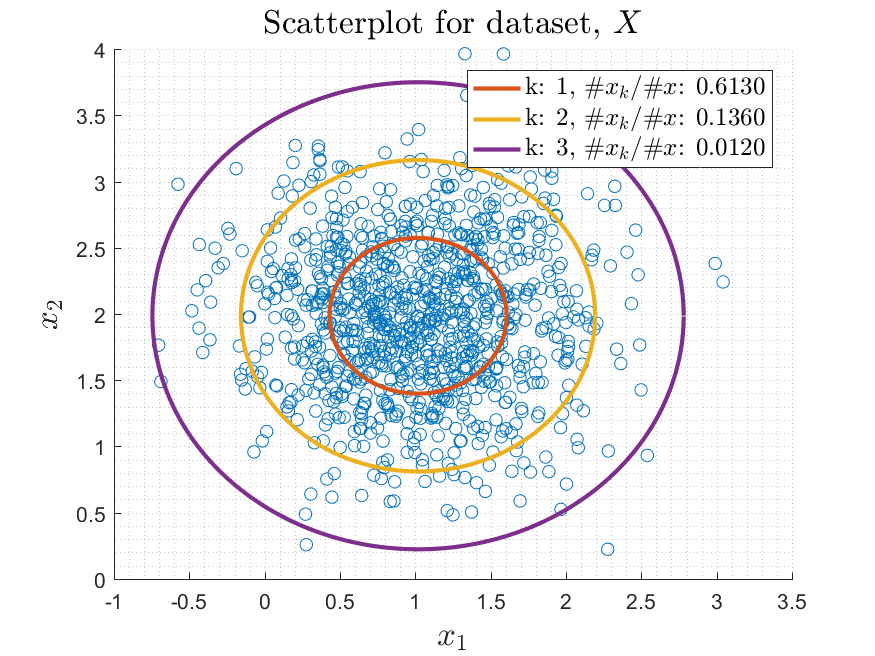
\includegraphics[width=0.65\textwidth]{Figures/plot2_1_scatter.png}	\caption{\label{fig:prob21}The dataset plotted with three circles with radius $k\sigma$, where $k\in {1,2,3}$ and $\sigma$ is the standard deviation of the given data.}
\end{figure}
The code implementation can be found in the enclosed folder \verb|code|.

\subsection*{Problem 2.2}

\begin{figure}[H]
    \centering
    \begin{subfigure}[b]{0.65\textwidth}
        \centering
        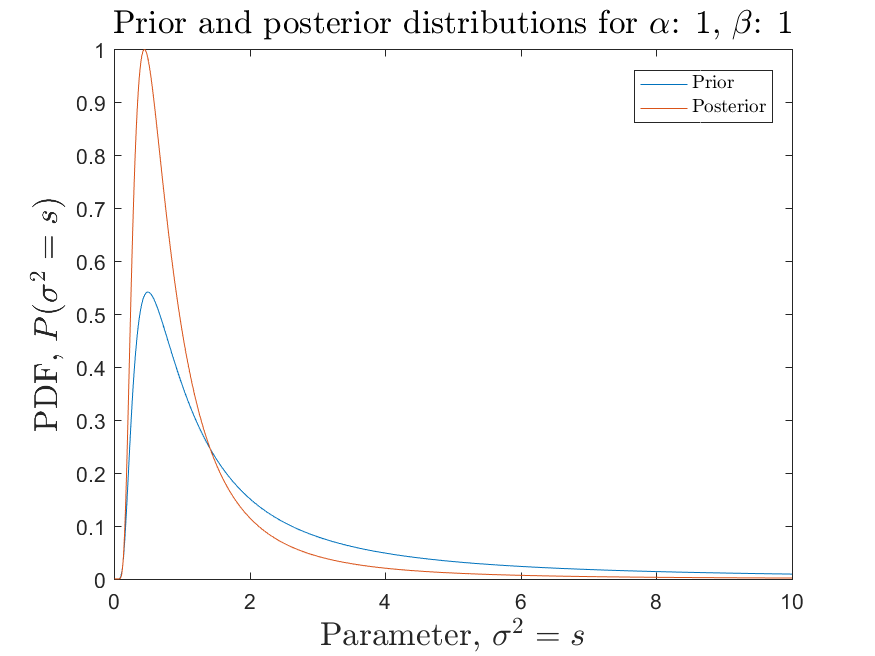
\includegraphics[width=\textwidth]{Figures/plot2_2_a1.png}
    \end{subfigure}
    \begin{subfigure}[b]{0.65\textwidth}
        \centering
        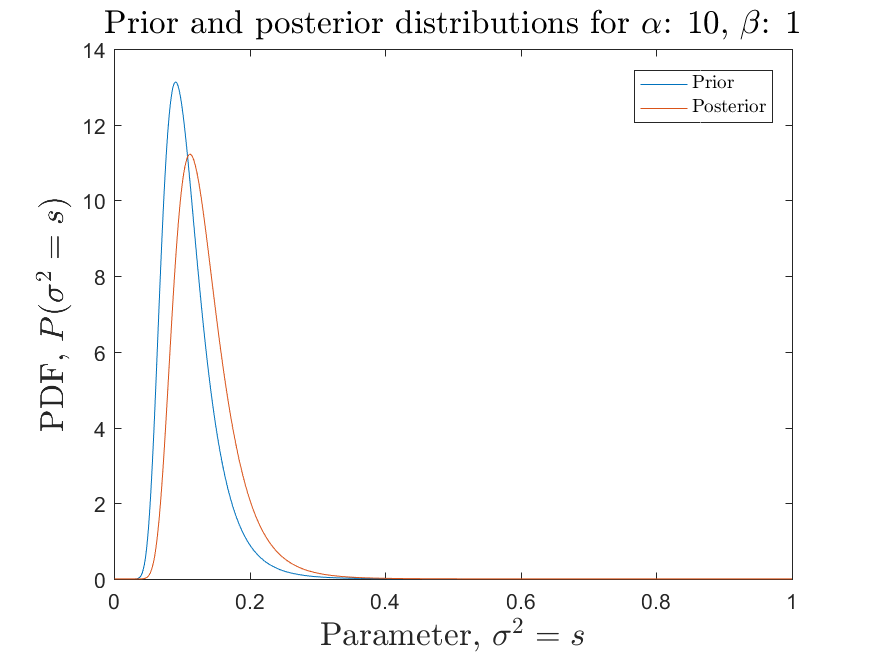
\includegraphics[width=\textwidth]{Figures/plot2_2_a2.png}
    \end{subfigure}
    \caption{\label{fig:distributions} The prior vs. posterior distribution using the given data for different hyperparameters $\alpha$ and $\beta$.}
\end{figure}

\begin{equation}
\sigma^2_{MAP}=\frac{\beta+\sigma^2_{MLE}}{\alpha+2}
\end{equation}


where

$\sigma^2_{MAP}$ derivation:

\begin{equation}
\sigma^2_{MAP}= \argmax_{\sigma^2=s}  p(s| x_1,...,x_n;\alpha,\beta)
\end{equation}

To find this we use the derivative

\begin{equation}
\begin{array}{rcl}
\frac{\partial }{\partial s} Gam(s|a,b) & = & \frac{\partial}{\partial s} \frac{b^a}{\Gamma(a)}s^{-a-1}\exp{\left(-\frac{b}{s}\right)} \\
& = & -\frac{b^as^{-a-3}e^{-\frac{b}{s}}(-b+as+s)}{\Gamma(a)}
\end{array}
\end{equation}

and we want to check when this is zero,

\begin{equation}
\frac{\partial}{\partial s}Gam(s|a,b) = 0
\end{equation}

we have two uninteresting cases, i.e. $s=0$ and $s\rightarrow \inf$. The only non-trivial case is when,

\begin{equation}
-b+(a+1)s=0 \Rightarrow s = \frac{b}{a+1}.
\end{equation}

Using $b=\beta+\frac{1}{2}\sigma^2_{MLE}$ and $a = \alpha +1$ we get

\begin{equation}
\sigma^2_{MAP;\alpha,\beta} = \frac{\beta + \frac{1}{2}\sigma^2_{MLE}}{\alpha+2}
\end{equation}

\begin{equation}
\sigma^2_{MLE}=\frac{1}{2}\left(x-\mu\right)^{T}\left(x-\mu\right)
\end{equation}

so we get,

\begin{equation}
\begin{array}{rrcl}
\alpha=1, \beta = 1 \Rightarrow & \sigma^2_{MAP} & = & 0.5292\\
\alpha=10, \beta = 1 \Rightarrow & \sigma^2_{MAP} & = & 0.1323
\end{array}
\end{equation}


\begin{equation}
B_{factor}=\frac{\sigma^2_{MAP;1}}{\sigma^2_{MAP;2}}=4
\end{equation}

so we would prefer the model using $\alpha=1$ and $\beta=1$.

\end{document}
